%=========================================================
% Capítulo 10 — Sistemas operacionais e exemplos reais
%=========================================================
\chapter{Sistemas operacionais e exemplos reais}
\label{ch:sistemas-operacionais}

\noindent\textbf{Resumo:}
Este capítulo descreve como os princípios teóricos da assimilação são implementados em sistemas operacionais reais.
São apresentados os principais esquemas usados em meteorologia — GSI, JEDI e LETKF — e o ciclo de assimilação típico que integra observações de satélite, superfície e sondagens.
Discute-se também o papel das observações convencionais e remotas, e como elas alimentam os modelos numéricos de previsão.

%---------------------------------------------------------
\section{O ciclo de assimilação}
Um \emph{ciclo de assimilação} representa a sequência de etapas que transforma dados observacionais em um estado inicial coerente para o modelo.
Cada ciclo compreende:
\begin{enumerate}
  \item previsão de curto prazo (\emph{forecast}) até o próximo tempo de análise;
  \item coleta e pré-processamento de observações;
  \item assimilação das observações no modelo;
  \item geração do campo analisado;
  \item reinício da próxima previsão.
\end{enumerate}
Em operação, esse ciclo é executado a cada 6 horas ou menos, garantindo que o sistema de previsão permaneça atualizado com as condições atmosféricas reais.

\begin{figure}[h!]
\centering
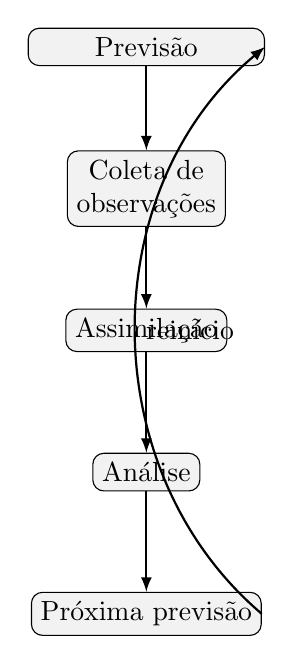
\begin{tikzpicture}[>=latex, node distance=1.8cm, every node/.style={align=center}]
  \node[draw,rounded corners,fill=gray!10,minimum width=3cm] (fc) {Previsão};
  \node[draw,rounded corners,fill=gray!10,below of=fc] (obs) {Coleta de\\observações};
  \node[draw,rounded corners,fill=gray!10,below of=obs] (assim) {Assimilação};
  \node[draw,rounded corners,fill=gray!10,below of=assim] (anal) {Análise};
  \node[draw,rounded corners,fill=gray!10,below of=anal] (next) {Próxima previsão};
  \draw[->,thick] (fc) -- (obs);
  \draw[->,thick] (obs) -- (assim);
  \draw[->,thick] (assim) -- (anal);
  \draw[->,thick] (anal) -- (next);
  \draw[->,thick,bend left=50] (next.east) to node[right]{reinício} (fc.east);
\end{tikzpicture}
\caption{Esquema conceitual do ciclo operacional de assimilação de dados.}
\label{fig:cycle}
\end{figure}

%---------------------------------------------------------
\section{O sistema GSI}
O \textbf{Gridpoint Statistical Interpolation} (GSI) é um dos sistemas mais difundidos de assimilação variacional.
Desenvolvido pelo NCEP (EUA), ele implementa as formas 3DVar e 4DEnVar.
Sua função custo segue a equação~\eqref{eq:J-3DVar}, e o processo é resolvido iterativamente usando o método de gradiente conjugado.

O GSI é amplamente utilizado no Brasil (INPE/CPTEC, SMNA) e em instituições internacionais (NOAA, NASA, JCSDA).
Ele assimila observações de superfície, sondagens, dados de satélite (radiâncias), vento derivado de imagens, GPSRO e perfis de umidade.
Cada tipo de observação é representado por um \emph{operador de observação} específico — parte essencial do código.

%---------------------------------------------------------
\section{O sistema JEDI}
O \textbf{Joint Effort for Data Assimilation Integration} (JEDI) é uma plataforma modular e moderna desenvolvida pelo \emph{Joint Center for Satellite Data Assimilation} (JCSDA).
Seu objetivo é unificar a assimilação para diferentes modelos (atmosfera, oceano, superfície) em uma estrutura comum orientada a objetos em C++/Fortran, com configuração em YAML.
Entre suas principais características:
\begin{itemize}
  \item arquitetura genérica e escalável;
  \item suporte a assimilação variacional e \emph{ensemble};
  \item integração com sistemas de observação via OOPS (Object-Oriented Prediction System);
  \item compilação automatizada via \texttt{spack-stack}.
\end{itemize}
O JEDI implementa os métodos 3DVar, 4DVar, EnKF e híbridos EnVar, tornando-se a principal base para o desenvolvimento futuro de sistemas comunitários como o \textbf{MONAN} no Brasil.

%---------------------------------------------------------
\section{O sistema LETKF}
O \textbf{Local Ensemble Transform Kalman Filter} (LETKF) é um esquema baseado em EnKF, mas aplicado localmente em cada ponto de grade.
Isso permite paralelismo massivo e menor custo de comunicação.
Cada subdomínio realiza sua própria análise com base em um pequeno subconjunto de observações próximas:
\[
\mathbf{x}_a^l = \mathbf{x}_b^l + \mathbf{K}_l (\mathbf{y}^l - \mathbf{H}_l \mathbf{x}_b^l),
\]
onde o índice $l$ representa uma região local.
A análise global é então recomposta pela junção contínua dos resultados locais.

O LETKF é utilizado em centros como JMA (Japão), ECMWF e em pesquisas no Brasil (CPTEC/INPE, IAG/USP), demonstrando excelente desempenho em modelos de alta resolução.

%---------------------------------------------------------
\section{Tipos de observações assimiladas}
Os sistemas operacionais incorporam uma ampla gama de dados:
\begin{itemize}
  \item \textbf{Observações de superfície:} estações meteorológicas, boias oceânicas, aeroportos (SYNOP, METAR, SHIP, BUOY);
  \item \textbf{Sondagens:} radiossondas, dropsondes, balões meteorológicos;
  \item \textbf{Satélites:} radiâncias (ATMS, AMSU-A, IASI, GOES-16), perfis de vento e umidade, GPSRO;
  \item \textbf{Radar meteorológico:} velocidade radial e refletividade;
  \item \textbf{Aviação e reanálises:} dados de aeronaves (AMDAR) e produtos compostos.
\end{itemize}
Essas observações passam por controles de qualidade e normalização antes de serem assimiladas.
O equilíbrio entre cobertura espacial e precisão é fundamental para o desempenho global do sistema.

%---------------------------------------------------------
\section{Exemplo prático: ciclo de 6 horas}
Em um sistema global típico (como o BAM + GSI do CPTEC), o ciclo de assimilação segue:
\begin{enumerate}
  \item \textbf{T\textsubscript{0}} – Coleta de observações entre T–3 h e T+3 h;
  \item \textbf{Análise} – Execução do GSI com os dados do período;
  \item \textbf{Integração} – Modelo BAM executado por 6 h;
  \item \textbf{Saída} – Resultado usado como background do próximo ciclo.
\end{enumerate}
Esse processo é automatizado em ambientes HPC com gerenciadores de filas (SLURM, PBS) e scripts de controle.

%---------------------------------------------------------
\section{Síntese}
Os sistemas operacionais (GSI, JEDI, LETKF) materializam a teoria da assimilação em fluxos de produção complexos e massivamente paralelos.
O sucesso da previsão numérica moderna depende da integração harmônica entre o modelo, o pré-processamento das observações e o ciclo de assimilação.
Esses sistemas são hoje o núcleo operacional de previsão e pesquisa em meteorologia.

% Fim do Capítulo 10
